\chapter{立体化学进阶}\label{ch:b1:stereochemistry-in-depth}

压碎几粒葛缕子籽，再碾一片留兰香叶，闻到的是两种截然不同的
气味。二者的主要气味物质都是香芹酮 \ce{C10H14O}，
原子种类与连接顺序完全相同——但两者互为镜像，
正如左手之于右手，鼻腔中的受体本身由镜像不对称的分子构成，
因而能将二者区分开来。
药物、香料与生命分子都具有三维结构，
忽略第三维度的结构式只能说明一半的问题。
本章介绍在空间中画出分子的工具，
无歧义地命名每一种排列方式，
追踪分子不断进行的转动，
并测量能够区分互为镜像的分子的那一种物理性质。

\begin{recall}
第 1 册（十二年级）介绍了手性分子、不对称碳原子、
对映异构体、$Z$/$E$ 异构体以及乙烷的构象。
碳原子四个键的四面体排布，以及单键与双键的
$\sigma$/$\pi$ 描述，均来自
\cref{ch:b1:lewis-resonance-vsepr}。
\end{recall}

\begin{omfigure}
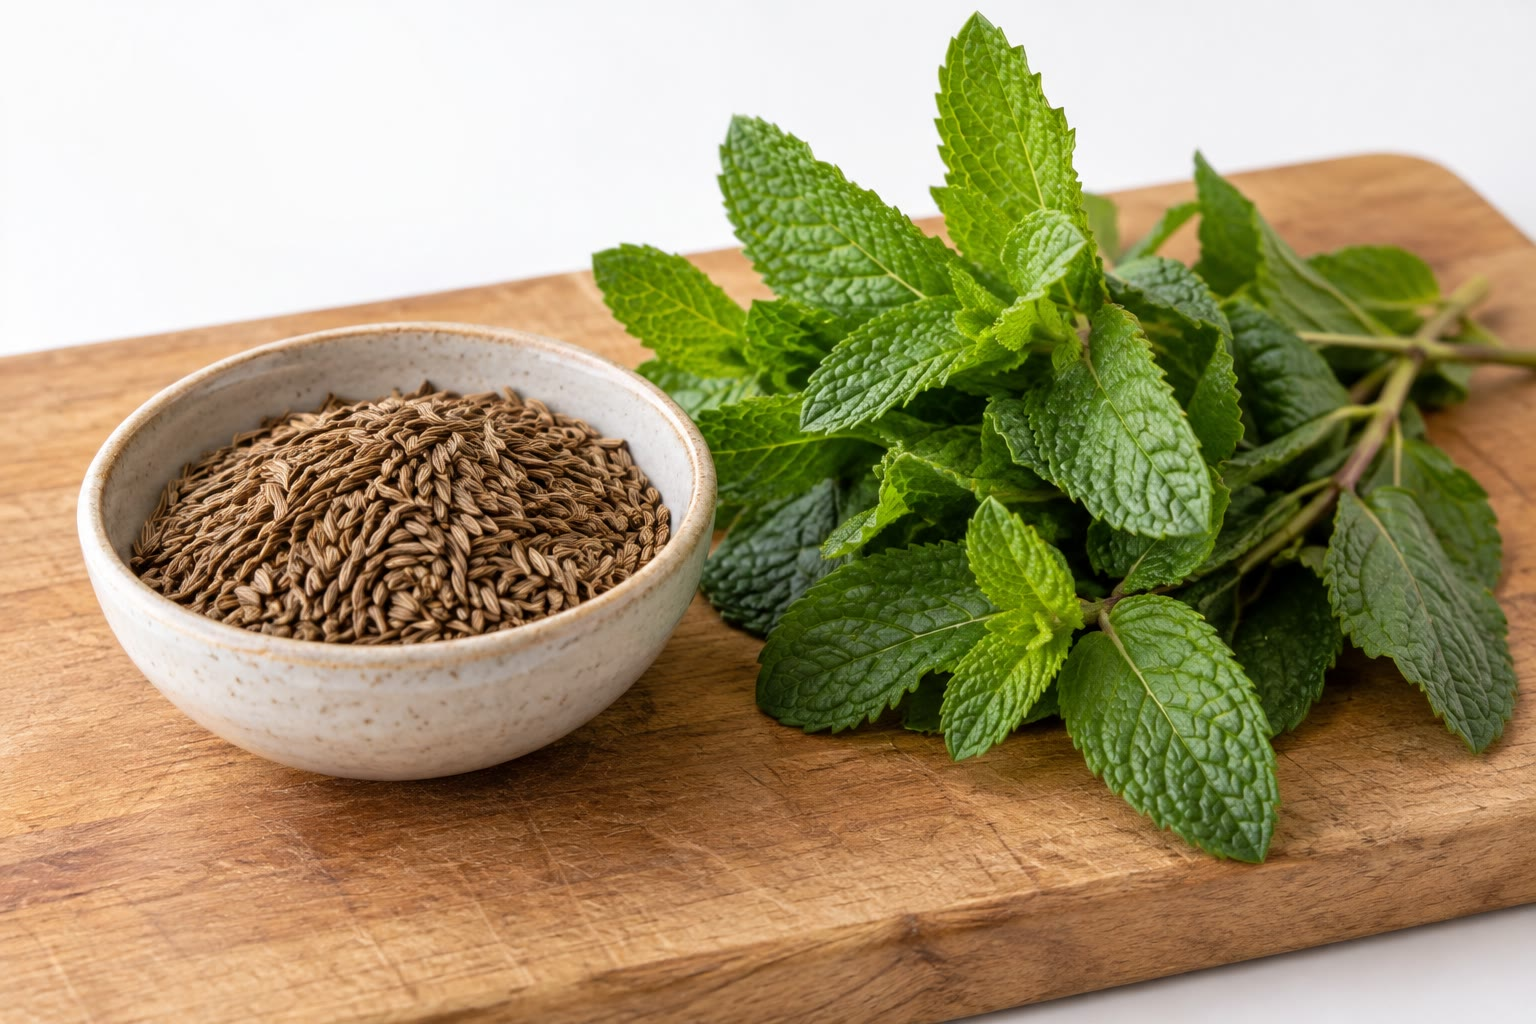
\includegraphics[width=0.55\linewidth]{images/book2/ai/b1-16-caraway-mint.jpg}

{\small 葛缕子籽与留兰香叶。葛缕子的气味主要源于
\cip{S}-香芹酮，留兰香则来自其镜像，\cip{R}-香芹酮。}
\end{omfigure}

\section{异构与表示法}

\begin{definition}[构造、构型与构象]\label{def:b1:stereochemistry-in-depth:isomers}
分子式相同、原子连接顺序不同的两种化合物称为
\emph{构造异构体}\index{构造异构体}。
构造相同、仅原子在空间中的排布不同的化合物，
称为\emph{立体异构体}\index{立体异构体}。
只有断开化学键才能改变的排布，称为立体异构体的
\emph{构型}\index{构型}；
绕单键旋转、不断开任何化学键即可得到的排布，
称为\emph{构象}\index{构象}。
\end{definition}

室温下，单键的旋转每秒可发生数十亿次，
构象之间迅速相互转化，无法分离；
而构型稳定，可得到不同的化合物。

\begin{definition}[表示法]\label{def:b1:stereochemistry-in-depth:representations}
在\emph{楔形式}\index{楔形式}中，两根键画在纸面内，
一根实楔形键指向读者，一根虚楔形键背离读者。
\emph{纽曼投影式}\index{纽曼投影式}沿一条 C--C 键观察分子：
前碳原子画成三根其余键交汇的一点，
后碳原子用一个圆表示，
其键自圆周引出。在\emph{费歇尔投影式}\index{费歇尔投影式}中，
碳链竖直排列，水平键指向读者，
竖直键背离读者；每个交叉点即为一个立体中心。
\end{definition}

\begin{omfigure}
\begin{tikzpicture}[font=\small]
  % staggered and eclipsed ethane, Newman
  \pic (s) at (0,0) {omnewman={90}{30}};
  \foreach \k in {1,2,3} { \node at (s-f\k) {H}; \node at (s-b\k) {H}; }
  \node at (0,-1.9) {交叉式};
  \pic (e) at (3.6,0) {omnewman={90}{108}};
  \foreach \k in {1,2,3} { \node at (e-f\k) {H}; }
  \foreach \k in {1,2,3} { \node[font=\scriptsize, black!60] at ($(e-b\k)!-0.12!(e-c)$) {H}; }
  \node at (3.6,-1.9) {重叠式};
  % Fischer projection of (R)-lactic acid
  \begin{scope}[xshift=7.6cm]
    \draw[thick] (-0.9,0) -- (0.9,0) (0,-0.9) -- (0,0.9);
    \node[above] at (0,0.9) {\ce{COOH}};
    \node[below] at (0,-0.9) {\ce{CH3}};
    \node[left] at (-0.9,0) {H};
    \node[right] at (0.9,0) {OH};
    \node at (0,-1.9) {费歇尔};
  \end{scope}
  % Cram of the same
  \begin{scope}[xshift=11.0cm]
    \node at (0,0) {\chemfig{C(-[2]COOH)(-[:210]H_3C)(<:[:-12]OH)(<[:-55]H)}};
    \node at (0,-1.9) {楔形式};
  \end{scope}
\end{tikzpicture}

{\small 左：乙烷沿 C--C 键的纽曼投影式，分别为交叉式
（后碳的键位于前碳的键之间）和重叠式（后碳的键被前碳的键遮住，
画时略作错开）。右：同一分子 \cip{R}-乳酸，
分别以费歇尔投影式与楔形式表示，
（费歇尔十字的竖直键背离读者，
水平键指向读者）。}
\end{omfigure}

\begin{method}[由楔形式到纽曼投影式]\label{met:b1:stereochemistry-in-depth:newman-from-cram}
\begin{enumerate}
  \item 选定所沿观察的键，并确定靠近观察者的一端。
  \item 从中心画出前碳的三根键，
        保持它们在观察者视线中的顺序（顺时针或逆时针）
        不变。
  \item 从圆周画出后碳的键，并保持
        从同一侧看去的顺序。
  \item 检验：后碳旋转 $60^\circ$ 时，由交叉式变为重叠式；
        旋转 $120^\circ$ 时，由一种交叉式构象
        变为下一种交叉式构象。
\end{enumerate}
\end{method}

\section{构型：CIP 规则}

\begin{definition}[CIP 规则与描述符]\label{def:b1:stereochemistry-in-depth:cip}
\emph{CIP 规则}\index{CIP 规则}（康–英戈尔德–普雷洛格）对立体中心的四个取代基进行排序：
原子序数大者优先；
若原子序数相同，则比较与其相连的原子集合，依次向外逐层比较；
双键视为与重复原子相连的两个单键。
将优先级最低的取代基背离视线，
若 $1 \to 2 \to 3$ 顺时针转动，则描述符为 \cip{R}，
逆时针则为 \cip{S}。对于碳原子上各连有两个取代基的双键，
若两个优先级较高的取代基位于同侧，则记为 \cip{Z}，
位于异侧则为 \cip{E}。
\end{definition}

\begin{method}[指定 \texorpdfstring{\cip{R}}{(R)} 或 \texorpdfstring{\cip{S}}{(S)}]\label{met:b1:stereochemistry-in-depth:cip}
\begin{enumerate}
  \item 按 CIP 规则对四个取代基排序。
  \item 若优先级最低的取代基背离观察者（虚楔形键，或费歇尔投影式中的竖直键），
        则直接读取
        $1 \to 2 \to 3$ 的转向。
  \item 若其指向观察者（实楔形键，或费歇尔投影式中的水平键），
        则读取转向，并将描述符对调。
  \item 交换任意两个取代基会使描述符反转：
        这是一种快速检验的办法。
\end{enumerate}
对于乳酸，$\ce{OH} > \ce{COOH} > \ce{CH3} > \ce{H}$（先比较 O；
C(O,O,O) 胜过 C(H,H,H)）。上图的费歇尔投影式中，H 为水平键
（指向观察者），$\ce{OH} \to \ce{COOH} \to \ce{CH3}$ 逆时针转动，
取反后，该中心为 \cip{R}。
\end{method}

\section{手性及其影响}

\begin{definition}[立体中心，手性]\label{def:b1:stereochemistry-in-depth:stereocentre}
若一个物体不能与其镜像叠合，则称它是\emph{手性}\index{手性}的，
否则称为\emph{非手性的}\index{非手性的}；这一性质称为
\emph{手性}\index{手性}。\emph{立体中心}\index{立体中心}是这样一种原子：
交换其上两个取代基可得立体异构体；
例如，四个取代基互不相同的四面体形碳原子，
即为一个立体中心。
\end{definition}

具有对称面或对称中心的分子是非手性的；
两者皆无的分子，在实际中通常是手性的。严格判据以对称操作表述，
见本科三年级分册。

\begin{definition}[对映异构体，非对映异构体，内消旋化合物，外消旋混合物]\label{def:b1:stereochemistry-in-depth:enantiomers}
互为镜像的两种立体异构体称为
\emph{对映异构体}\index{对映异构体}；彼此不为镜像的立体异构体称为
\emph{非对映异构体}\index{非对映异构体}。一种具有立体中心而非手性的
化合物称为\emph{内消旋化合物}\index{内消旋化合物}。
等物质的量的两种对映异构体的混合物称为
\emph{外消旋混合物}\index{外消旋混合物}。
\end{definition}

\begin{proposition}[立体异构体的数目]\label{prop:b1:stereochemistry-in-depth:max-stereoisomers}
含 $n$ 个立体中心（且无其他立体单元）的分子，
至多有 $2^n$ 种立体异构体，至多组成 $2^{n-1}$ 对
对映异构体；存在内消旋化合物时，数目更少。
\end{proposition}

\begin{proof}
每个中心独立地取 \cip{R} 或 \cip{S}，共有 $2^n$ 种组合。
镜像会改变每个描述符，因此这些组合两两配对，
形成 $2^{n-1}$ 对对映异构体。若某一组合经分子转动后与自身的镜像重合（即内消旋体），
则其所在的一对
缩并为一种化合物。
\end{proof}

酒石酸 \ce{HOOC-CH(OH)-CH(OH)-COOH} 具有两个等价的中心：
\cip{R,R} 与 \cip{S,S} 互为对映异构体，而 \cip{R,S} 在两个碳原子之间
有一个对称面，为内消旋化合物，共三种立体异构体，而非四种。

\begin{proposition}[对映异构体的性质]\label{prop:b1:stereochemistry-in-depth:enantiomer-properties}
一对对映异构体的熔点和沸点相同，在非手性溶剂中的溶解度，
光谱以及与非手性试剂的反应活性也相同；
二者对偏振光的作用不同，与其他手性分子的相互作用
也不同。非对映异构体的
各项性质均不相同。
\end{proposition}

\begin{proof}
凡只依赖于分子内部，或分子与非手性伙伴之间的距离与角度的性质，
对物体及其镜像都相同，
因为反射保持距离与角度不变。
手性伙伴（如受体、手性试剂，或下文所述偏振光的螺旋路径）
所形成的配对是非对映的，不再互为镜像，因而性质有所不同。
非对映异构体不能由任何反射相互得到：
它们的内部距离并不相同。
\end{proof}

\begin{omfigure}
\begin{tikzpicture}[font=\small, line join=round]
  \foreach \dx/\kind/\lab in {0/1/{\cip{R}-香芹酮（留兰香）}, 5.2/0/{\cip{S}-香芹酮（葛缕子）}} {
  \begin{scope}[xshift=\dx cm]
    \coordinate (c1) at (0,1); \coordinate (c2) at (0.87,0.5);
    \coordinate (c3) at (0.87,-0.5); \coordinate (c4) at (0,-1);
    \coordinate (c5) at (-0.87,-0.5); \coordinate (c6) at (-0.87,0.5);
    \draw[thick] (c1) -- (c2) -- (c3) -- (c4) -- (c5) -- (c6) -- cycle;
    \draw[thick] ($(c2)!0.15!(c3)+(-0.12,0)$) -- ($(c3)!0.15!(c2)+(-0.12,0)$);
    \draw[thick] (c1) -- ++(0,0.7) node[above] {O};
    \draw[thick] ($(c1)+(0.1,0)$) -- ++(0,0.62);
    \draw[thick] (c2) -- ++(0.75,0.43) node[right] {\ce{CH3}};
    \coordinate (q) at ($(c5)+(-0.75,-0.43)$);
    \ifnum\kind=1
      \fill (c5) -- ($(q)+(0.06,-0.1)$) -- ($(q)+(-0.06,0.1)$) -- cycle;
    \else
      \foreach \t in {0.15,0.3,0.45,0.6,0.75,0.9}
        \draw ($(c5)!\t!(q)+(\t*0.06,-\t*0.1)$) -- ($(c5)!\t!(q)+(-\t*0.06,\t*0.1)$);
    \fi
    \draw[thick] (q) -- ++(-0.6,0.5) node[above] {\ce{CH2}};
    \draw[thick] ($(q)+(0.08,0.06)$) -- ++(-0.6,0.5);
    \draw[thick] (q) -- ++(0,-0.75) node[below] {\ce{CH3}};
    \node[font=\scriptsize] at ($(c5)+(0.35,0.12)$) {5};
    \node at (0,-2.85) {\lab};
  \end{scope}}
\end{tikzpicture}

{\small 两种香芹酮按同一骨架绘出：C5 上的异丙烯基
在其中一种中指向读者（实楔形键），在另一种中背离读者（虚楔形键），
C5 上的氢（未画出）位于相反一侧。
它们互为镜像：是对映异构体
（见\cref{exo:b1:stereochemistry-in-depth:4}）。}
\end{omfigure}

\begin{history}[四面体碳原子]
\begin{minipage}[t]{0.2\linewidth}\vspace{0pt}
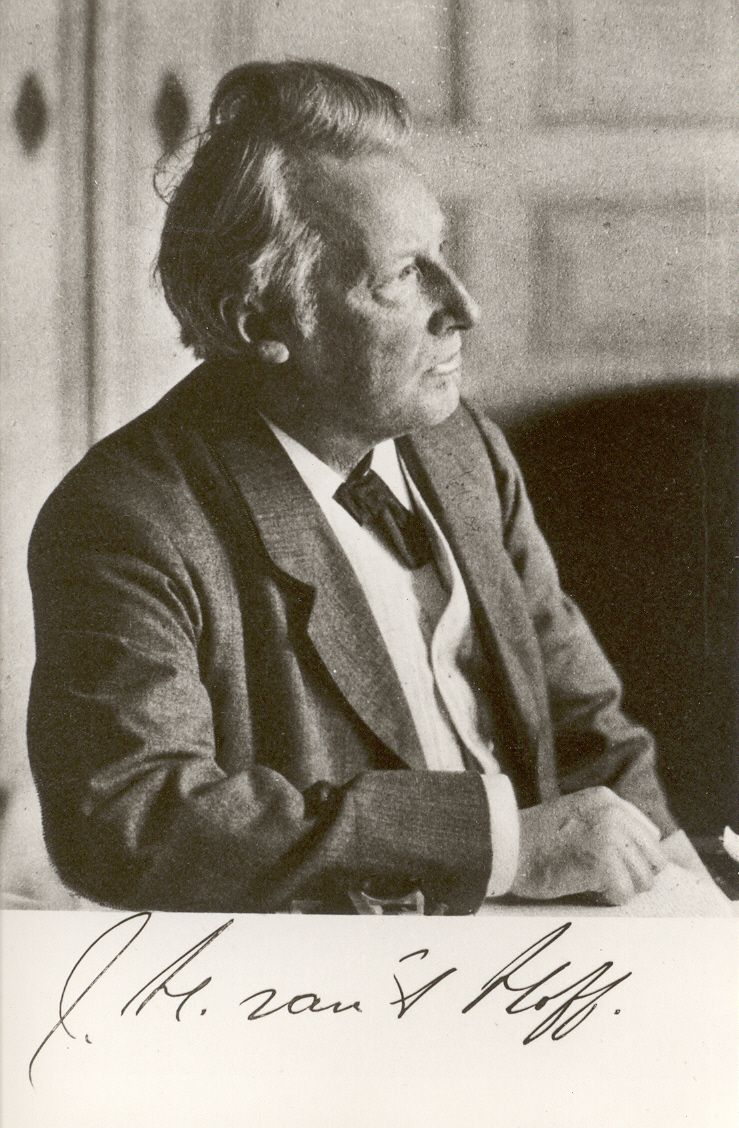
\includegraphics[width=\linewidth]{images/book2/van-t-hoff.jpg}
\end{minipage}\hfill
\begin{minipage}[t]{0.76\linewidth}\vspace{0pt}
年轻化学家雅各布斯·亨里库斯·范托夫提出，碳原子的四个
键指向四面体的顶点。含四个不同取代基的碳
原子于是存在两种互为镜像的排布，
这解释了为何某些化合物存在两种形式，
它们仅在使偏振光旋转的方式上不同。这一思想是
本章所有绘图的出发点。
（照片发表于 1911 年，公有领域，维基共享资源。）
\end{minipage}
\end{history}

\section{构象}

\begin{definition}[扭转角与构象]\label{def:b1:stereochemistry-in-depth:conformations}
对于四个原子 A--B--C--D，绕 B--C 的\emph{扭转角}\index{扭转角}
$\theta$ 是平面 ABC 与 BCD 所成的夹角，在沿 B--C 的纽曼投影式上读出。
当前、后碳原子的键在投影中对齐时，构象称为
\emph{重叠式构象}\index{重叠式构象}；当二者交替排列时，
构象称为\emph{交叉式构象}\index{交叉式构象}。在丁烷中，
沿 C2--C3 观察，两甲基位于 $180^\circ$ 的交叉式构象
称为\emph{对位交叉构象}\index{对位交叉构象}，
两甲基位于 $\pm 60^\circ$ 时，
构象为\emph{邻位交叉构象}\index{邻位交叉构象}。
在环己烷中，无张力的皱折环为\emph{椅式构象}\index{椅式构象}；
每个碳原子带有一个\emph{直立键}\index{直立键}，
与环轴平行，
另有一个\emph{平伏键}\index{平伏键}，大致位于环的平均平面内。
\emph{环翻转}\index{环翻转}使一种椅式构象
转变为另一种，每个直立键变为平伏键，
反之亦然。
\end{definition}

\begin{omfigure}
\begin{tikzpicture}
\begin{axis}[
  width=0.82\linewidth, height=5.8cm, xmin=0, xmax=360, ymin=0, ymax=21,
  legend style={font=\scriptsize, draw=none, at={(0.5,0.62)}, anchor=center},
  axis x line=bottom, axis y line=left, xlabel={扭转角 $\theta$（度）},
  ylabel={能量 (kJ/mol)}, xtick={0,60,120,180,240,300,360},
  tick label style={font=\small}, label style={font=\small}]
\addplot[omDef, very thick] table[x=theta, y=butane] {figdata/out/bachelor-1-butane-torsion.dat};
\addplot[omProp, thick, dashed] table[x=theta, y=ethane] {figdata/out/bachelor-1-butane-torsion.dat};
\node[font=\scriptsize, anchor=south west] at (axis cs:0,18.4) {顺式};
\node[font=\scriptsize, anchor=south] at (axis cs:62,18.4) {邻位交叉};
\node[font=\scriptsize, anchor=south] at (axis cs:120,18.4) {重叠};
\node[font=\scriptsize, anchor=south] at (axis cs:180,18.4) {对位交叉};
\node[font=\scriptsize, anchor=south] at (axis cs:240,18.4) {重叠};
\node[font=\scriptsize, anchor=south] at (axis cs:298,18.4) {邻位交叉};
\node[font=\scriptsize, anchor=south east] at (axis cs:360,18.4) {顺式};
\legend{丁烷, 乙烷}
\end{axis}
\end{tikzpicture}

{\small 丁烷绕中心键的扭转能（实线；$\theta
= 0$ 时两甲基相互重叠），以及乙烷的扭转能（虚线），
由实验扭转势计算得出。乙烷势垒：
\qty{12.2}{kJ/mol}。丁烷：对位交叉最稳定；邻位交叉高出 \qty{2.8}{kJ/mol}，
位于 $\theta = 62^\circ$ 处；势垒 \qty{15.2}{kJ/mol}（甲基
与氢重叠），以及 \qty{16.5}{kJ/mol}（甲基与甲基重叠）。}
% ledger: rot:ethane-V3, rot:butane-V1, rot:butane-V2, rot:butane-V3, rot:butane-V4, rot:butane-V5, rot:butane-V6 (curves in figdata/bachelor-1/butane-torsion.py)
\end{omfigure}

与碰撞中可利用的热能相比，这些势垒很小
（$RT = \qty{2.5}{kJ/mol}$ 为室温下的值，分布尾部远大于此，
见\cref{ch:b1:elementary-steps}）：转动很快，
丁烷是对位交叉与邻位交叉分子的混合物，
二者无法分离。

\begin{method}[画椅式构象]\label{met:b1:stereochemistry-in-depth:draw-chair}
\begin{enumerate}
  \item 画两条平行线，向右微微向下倾斜，
        彼此错开；在左端用一个 V 形、右端用一个倒 V 形连接两线端点，
        以闭合六元环。
  \item 直立键竖直：朝上的碳原子上向上画，朝下的向下画，
        沿环交替排列。
  \item 平伏键与隔一个的环键平行，
        并指向外侧。
  \item 要翻转环，画出另一种椅式构象；
        在一种构象中为直立键的取代基，在另一种中为平伏键。
\end{enumerate}
\end{method}

\begin{omfigure}
\begin{tikzpicture}[font=\small]
  \pic (a) at (0,0) {omchair};
  \foreach \k in {1,2,3,4,5,6} \draw[omProp, thick] (a-c\k) -- (a-a\k);
  \foreach \k in {1,2,3,4,5,6} \draw[omDef, thick] (a-c\k) -- (a-e\k);
  \node[omProp, anchor=south] at (a-a3) {直立键};
  \node[omDef, anchor=north] at (a-e5) {平伏键};
  \begin{scope}[xshift=4.9cm]
    \pic (b) at (0,0) {omchair};
    \draw[thick] (b-c1) -- (b-e1) node[right] {\ce{CH3}};
    \draw[thick] (b-c1) -- (b-a1) node[above] {H};
    \node at (0,-1.5) {平伏 \ce{CH3}};
  \end{scope}
  \draw[<->, thick] (8.1,0) -- (8.8,0) node[midway, above] {翻转};
  \begin{scope}[xshift=10.45cm]
    \pic (c) at (0,0) {omchairflip};
    \draw[thick] (c-c4) -- (c-a4) node[below] {\ce{CH3}};
    \draw[thick] (c-c4) -- (c-e4) node[right] {H};
    \node at (0,-1.5) {直立 \ce{CH3}};
  \end{scope}
\end{tikzpicture}

{\small 左：环己烷的椅式构象，六个直立键（橙色，
上下交替）和六个平伏键（蓝色）。右：甲基环己烷的两种
椅式构象，二者通过环翻转互相转化；甲基
在一种构象中为平伏键，在另一种中为直立键。}
\end{omfigure}

\begin{proposition}[平伏取代基更稳定]\label{prop:b1:stereochemistry-in-depth:chair-substituent}
在一取代环己烷中，取代基处于平伏键的椅式
构象更稳定。对甲基而言，直立位置会增加
与环碳原子之间的两个邻位交叉相互作用，每个的代价与丁烷相同
（\qtyrange{2.8}{2.9}{kJ/mol}），合计约 \qty{5.7}{kJ/mol}：
这是能量差的一个估计值。
\end{proposition}

\begin{proof}
沿 C1--C2 键观察，C1 上的直立甲基与环上的 C3 呈邻位交叉；
沿 C1--C6 键观察则与 C5 呈邻位交叉：两个类似丁烷的邻位交叉相互作用，
这也可看作甲基与 C3 和 C5 上的直立氢原子的拥挤
（1,3-二直立相互作用）。
平伏甲基与 C3 和 C5 呈对位交叉。每个邻位交叉相互作用的代价，
与丁烷中相同，为图中扭转势能给出的
\qty{2.8}{kJ/mol}。
\end{proof}

取 $\Delta E = \qty{5.7}{kJ/mol}$，于 \qty{25}{\celsius} 下，平伏与直立椅式构象之比为
$\exp(\Delta E/RT) = 10$，即约
\qty{91}{\percent} 为平伏构象（\cref{exo:b1:stereochemistry-in-depth:9}）。
体积较大的基团，如叔丁基，会将环锁定在
其处于平伏键的椅式构象中。

\section{旋光性}

\begin{definition}[旋光性，比旋光度]\label{def:b1:stereochemistry-in-depth:optical-activity}
若某物质能使通过其中的线偏振光的偏振面
发生旋转，则称该物质具有\emph{旋光性}\index{旋光性}。
面向光源观察，使偏振面顺时针旋转的物质称为
\emph{右旋的}\index{右旋的}物质，记为 $(+)$；
使偏振面逆时针旋转的称为\emph{左旋的}\index{左旋的}，记为
$(-)$。\emph{比旋光度}\index{比旋光度}为 $[\alpha] = \alpha/(\ell c)$，
其中 $\alpha$ 为测得的角度（以度计），$\ell$ 为光程（以分米计），
$c$ 为质量浓度，
单位为 \unit{g/mL}；它依赖于波长（通常取黄色钠光）、
温度和溶剂。
\end{definition}

\begin{omfigure}
\begin{tikzpicture}[font=\small, >={Stealth}]
  \fill[yellow!70!orange] (0,0) circle (0.25);
  \node[below] at (0,-0.45) {灯};
  \draw[thick] (1.3,-0.7) rectangle (1.45,0.7); \node[below] at (1.37,-0.75) {起偏器};
  \draw[omDef!20, fill=omDef!10] (2.4,-0.45) rectangle (5.6,0.45);
  \node at (4.0,0) {样品，长度 $\ell$};
  \draw[thick] (6.5,-0.7) rectangle (6.65,0.7); \node[below] at (6.57,-0.75) {检偏器};
  \draw (7.6,0) circle (0.3); \node[below] at (7.6,-0.45) {眼睛};
  \draw[->, orange!80!black] (0.3,0) -- (1.25,0);
  \draw[->, orange!80!black] (1.5,0) -- (2.35,0);
  \draw[->, orange!80!black] (5.65,0) -- (6.45,0);
  % polarisation planes
  \draw[thick, omThm] (1.9,-0.35) -- (1.9,0.35);
  \draw[thick, omThm] (6.05,-0.33) -- ++(70:0.0) -- (5.93,0.33);
  \draw[->, omThm] (5.75,0.55) arc[start angle=100, end angle=70, radius=0.6];
  \node[omThm, above] at (6.1,0.75) {$\alpha$};
\end{tikzpicture}

{\small 旋光仪。起偏器只允许在一个
平面内振动的光通过；手性样品使该平面转过 $\alpha$ 角；检偏器
转到光再次消失的位置，由此测得 $\alpha$。}
\end{omfigure}

\begin{proposition}[毕奥定律]\label{prop:b1:stereochemistry-in-depth:biot}
对于若干种旋光性溶质组成的稀溶液，旋转角具有可加性，
即 $\alpha = \ell\sum_i [\alpha]_i c_i$（\emph{毕奥定律}\index{毕奥定律}）。
两种对映异构体的比旋光度符号相反；
外消旋混合物不使光发生旋转。
\end{proposition}

\begin{proof}
稀溶液中，每种溶质独立作出贡献，
其贡献与光穿过的分子数成正比，即与 $\ell c_i$ 成正比；这
正是定律的实验内容。镜面反射使顺时针变为
逆时针：镜像分子使偏振面转过相反的角度，
在外消旋混合物中两部分贡献相互抵消。
\end{proof}

对总浓度为 $c$ 的两种对映异构体混合物，设 $x$ 为 $(-)$ 形式所占的分数，
则 $\alpha = \ell c[\alpha]_{(-)}(x - (1 - x)) =
\ell c[\alpha]_{(-)}(2x - 1)$，测得 $\alpha$ 即可确定组成。
旋光方向与构型描述符之间没有简单的对应关系：一个
\cip{R} 构型的化合物可能是 $(+)$ 或 $(-)$；留兰香中的 \cip{R}-香芹酮是
左旋的。

\section{练习}

\begin{exercise}[$\star$]\label{exo:b1:stereochemistry-in-depth:1}
判断下列每组化合物属于构造异构体、对映异构体、非对映异构体，
还是同一化合物的两种构象：丁-1-醇与丁-2-醇；
\cip{R}-与 \cip{S}-丁-2-醇；\cip{Z}-与 \cip{E}-丁-2-烯；丁烷的对位交叉构象与
邻位交叉构象；\cip{R,R}-与 \cip{R,S}-
酒石酸。
\end{exercise}

\begin{exercise}[$\star$]\label{exo:b1:stereochemistry-in-depth:2}
按 CIP 规则给下列基团排序：\ce{-OH}、\ce{-NH2}、\ce{-CH3}、\ce{-H}；再给
\ce{-CH2OH}、\ce{-CHO}、\ce{-COOH}、\ce{-CH(CH3)2} 排序；然后是
\ce{-Cl}、\ce{-CH2Cl}、\ce{-CCl3}、\ce{-Br}。
\end{exercise}

\begin{exercise}[$\star$]\label{exo:b1:stereochemistry-in-depth:3}
求 2,3-二氯丁烷、2-溴-3-氯丁烷
与戊-2,4-二醇各有多少种立体异构体，并指出其中的内消旋化合物。
\end{exercise}

\begin{exercise}[$\star$]\label{exo:b1:stereochemistry-in-depth:4}
按 CIP 规则给香芹酮 C5 上的四个取代基排序，并核对
图中给出的两个香芹酮的构型描述符（实楔形线：
异丙烯基指向读者，H 背离读者）。
\end{exercise}

\begin{exercise}[$\star\star$]\label{exo:b1:stereochemistry-in-depth:5}
画出丁烷沿 C2--C3 键的纽曼投影式，取 $\theta = 0$、60、
120 和 $180^\circ$ 时的构象，并在曲线上读出其能量。
若邻位交叉与对位交叉的能量相等，则处于邻位交叉构象的分子所占的分数为多少？
\end{exercise}

\begin{exercise}[$\star\star$]\label{exo:b1:stereochemistry-in-depth:6}
画出 \cip{S}-丙氨酸的费歇尔投影式，
\ce{H2N-CH(CH3)-COOH}，羧基在上。
氨基位于哪一侧？
\end{exercise}

\begin{exercise}[$\star\star$]\label{exo:b1:stereochemistry-in-depth:7}
证明 \textit{cis}-1,2-二甲基环己烷在两种椅式构象中均为一个甲基直立、
另一个甲基平伏，而 \textit{trans} 异构体在一种椅式构象中
两个甲基均为平伏键。哪一种异构体更稳定？请使用
本章中的估算方法。
\end{exercise}

\begin{exercise}[$\star\star$]\label{exo:b1:stereochemistry-in-depth:8}
某手性化合物的溶液，浓度为 \qty{0.100}{g/mL}，置于 \qty{2.00}{dm}
长的旋光管中，使光旋转 $+13.2^\circ$。求 $[\alpha]$。若改用
\qty{1.00}{dm} 的旋光管，结果会如何？相同浓度下的对映体又如何？
\end{exercise}

\begin{exercise}[$\star\star$]\label{exo:b1:stereochemistry-in-depth:9}
取 $\Delta E = \qty{5.7}{kJ/mol}$，并利用玻尔兹曼比值
$\exp(\Delta E/RT)$，计算甲基环己烷的椅式构象中，甲基处于
平伏键的构象所占的分数，温度分别为 \qty{25}{\celsius} 和 \qty{-50}{\celsius}。
\end{exercise}

\begin{exercise}[$\star\star\star$]\label{exo:b1:stereochemistry-in-depth:10}
解释为何乙烷只有一种交叉式构象，而丁烷有两种
（对位交叉和邻位交叉），并说明邻位交叉为何较不稳定。利用
图中的能量，估算丁烷在 \qty{25}{\celsius} 下的
对位交叉与邻位交叉的布居比（邻位交叉有两种构象，对位交叉有一种）。
\end{exercise}

\begin{exercise}[$\star\star\star$]\label{exo:b1:stereochemistry-in-depth:11}
考虑 2,3,4-三羟基戊二酸，
\ce{HOOC-CH(OH)-CH(OH)-CH(OH)-COOH}。数出其中的立体中心，证明
中心碳原子只有在两端的两个碳原子具有
相反的描述符时才是立体中心（假不对称），并数出
立体异构体的数目（包括内消旋化合物）。
\end{exercise}

\begin{exercise}[$\star\star\star$]\label{exo:b1:stereochemistry-in-depth:12}
某化合物一种对映体的样品（纯化合物在所用条件下 $[\alpha] = +66.0^\circ$）
已部分外消旋化：在
\qty{0.050}{g/mL} 浓度、\qty{1.00}{dm} 旋光管中测得 $+2.31^\circ$。
求两种对映体的分数。
\end{exercise}

\section{问题：薄荷醇，清凉的分子}

\begin{problem}[{周末问题——薄荷醇的三个立体中心，
其八种立体异构体，全平伏键的椅式构象，毕奥定律，以及
部分外消旋化样品中 (\textminus)-薄荷醇的百分含量}]
\label{pb:b1:stereochemistry-in-depth:1}
薄荷醇（2-异丙基-5-甲基环己-1-醇）赋予薄荷
清凉的口感。天然化合物为 $(-)$-薄荷醇，其构型为
\cip{1R,2S,5R}。实验室使用旋光仪测量（钠光谱线，
\qty{25}{\celsius}，溶剂为乙醇，$\ell = \qty{1.00}{dm}$）：其参比样品
为纯 $(-)$-薄荷醇，在 $c = \qty{0.0500}{g/mL}$ 时测得 $\alpha =
-2.46^\circ$；待测样品在相同浓度下测得
$-1.97^\circ$。

\medskip
第一部分——立体中心。
\begin{enumerate}
  \item 画出薄荷醇的构造式，并标出立体中心碳原子。
  \item 可能存在多少种立体异构体？有多少对
        对映异构体？
  \item 为何不存在内消旋化合物？
  \item 按 CIP 规则对 C1 上的取代基排序。
  \item 对 C2 上的取代基排序。
  \item 对 C5 上的取代基排序。
  \item 写出 $(-)$-薄荷醇的对映体的构型。
\end{enumerate}

\medskip
第二部分——椅式构象。
\begin{enumerate}[resume]
  \item 画出环己烷的一种椅式构象，使 $(-)$-薄荷醇的三个取代基
        全部置于平伏键。验证这与薄荷醇的
        相对构型（1,2-\textit{trans} 与 1,5-\textit{cis}）
        相符。
  \item 翻转后的椅式构象中，三个取代基怎样变化？
  \item 利用本章对一个直立甲基的估算，解释
        为何薄荷醇几乎全部处于同一种椅式构象。
  \item 新薄荷醇仅在 C1 上与薄荷醇有所不同，它是薄荷醇的
        对映异构体还是非对映异构体？
  \item 在新薄荷醇较稳定的椅式构象中，哪个基团为直立键？
  \item 为何薄荷醇与新薄荷醇的沸点不同，
        而薄荷醇的两种对映体的沸点却相同？
\end{enumerate}

\medskip
第三部分——旋光。
\begin{enumerate}[resume]
  \item 计算参比样品的 $[\alpha]$，并与手册给出的范围
        $-45^\circ$ 至 $-51^\circ$ 相比较，此范围针对 $(-)$-薄荷醇。
  \item $[\alpha]$ 对 $(+)$-薄荷醇应为多少？对外消旋薄荷醇呢？
  \item 计算待测样品的 $[\alpha]$。
  \item 写出两种对映体混合物的毕奥定律表达式，其中 $x$
        为 $(-)$-薄荷醇的分数。
  \item 将 $x$ 表示为测得旋光度与
        参比旋光度的函数。
  \item 另一种化合物的手性杂质能否使
        测量结果失真？请给出一种检验方法。
\end{enumerate}

\medskip
第四部分——组成。
\begin{enumerate}[resume]
  \item 计算待测样品中 $(-)$-薄荷醇的分数。
  \item 第二家供应商的样品在相同条件下测得 $-2.40^\circ$，
        试计算其组成。
  \item 哪一个样品更接近天然薄荷醇？
  \item 若改用 \qty{2.00}{dm} 旋光管，待测样品将给出多大的旋光角，
        并说明为何较长的旋光管更好？
  \item 写出待测样品中 $(-)$-薄荷醇的百分含量，
        保留三位有效数字。
\end{enumerate}
\end{problem}
